\documentclass{standalone}
\usepackage{tikz}
\usepackage{ctex,siunitx}
\setCJKmainfont{Noto Serif CJK SC}
\usepackage{tkz-euclide}
\usepackage{amsmath}
\usetikzlibrary{patterns, calc}
\usetikzlibrary {decorations.pathmorphing, decorations.pathreplacing, decorations.shapes,}

\begin{document}
\small
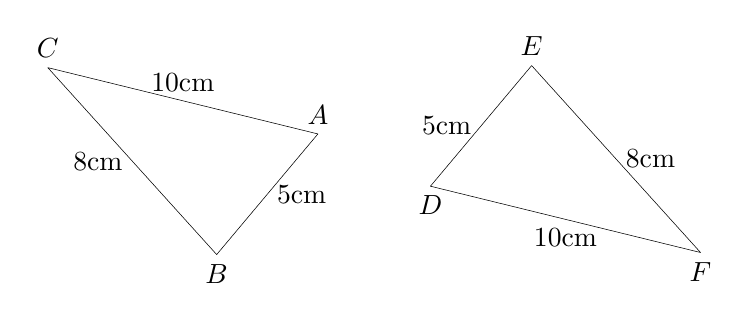
\begin{tikzpicture}[>=stealth,scale=0.8]
  \tkzSetUpPoint[fill=black]
  % \useasboundingbox(-1,-0.75)rectangle(3.7,1.4);
  \begin{scope}[rotate=50]
  \tkzDefPoints{0/0/B, 2.5/0/A}
  \tkzDefPoint(82.1:4){C}
  \tkzDrawPolygon(A,B,C)
  \tkzLabelPoints[above](A,C)
  \tkzLabelPoints[below](B)
  \tkzLabelSegment[above](A,C){10cm}
  \tkzLabelSegment[left](B,C){8cm}
  \tkzLabelSegment[right](A,B){5cm}
  \end{scope}
  \begin{scope}[xshift=5cm, yshift=3cm, rotate=-130]
    \tkzDefPoints{0/0/E, 2.5/0/D}
  \tkzDefPoint(82.1:4){F}
  \tkzDrawPolygon(D,E,F)
  \tkzLabelPoints[above](E)
  \tkzLabelPoints[below](D,F)
  \tkzLabelSegment[below](D,F){10cm}
  \tkzLabelSegment[right](E,F){8cm}
  \tkzLabelSegment[left](D,E){5cm}
  \end{scope}
\end{tikzpicture}
\end{document}